\chapter{Introduction and Overview}
\label{intro}

\section{How to use Z-Way}

\begin{figure} 
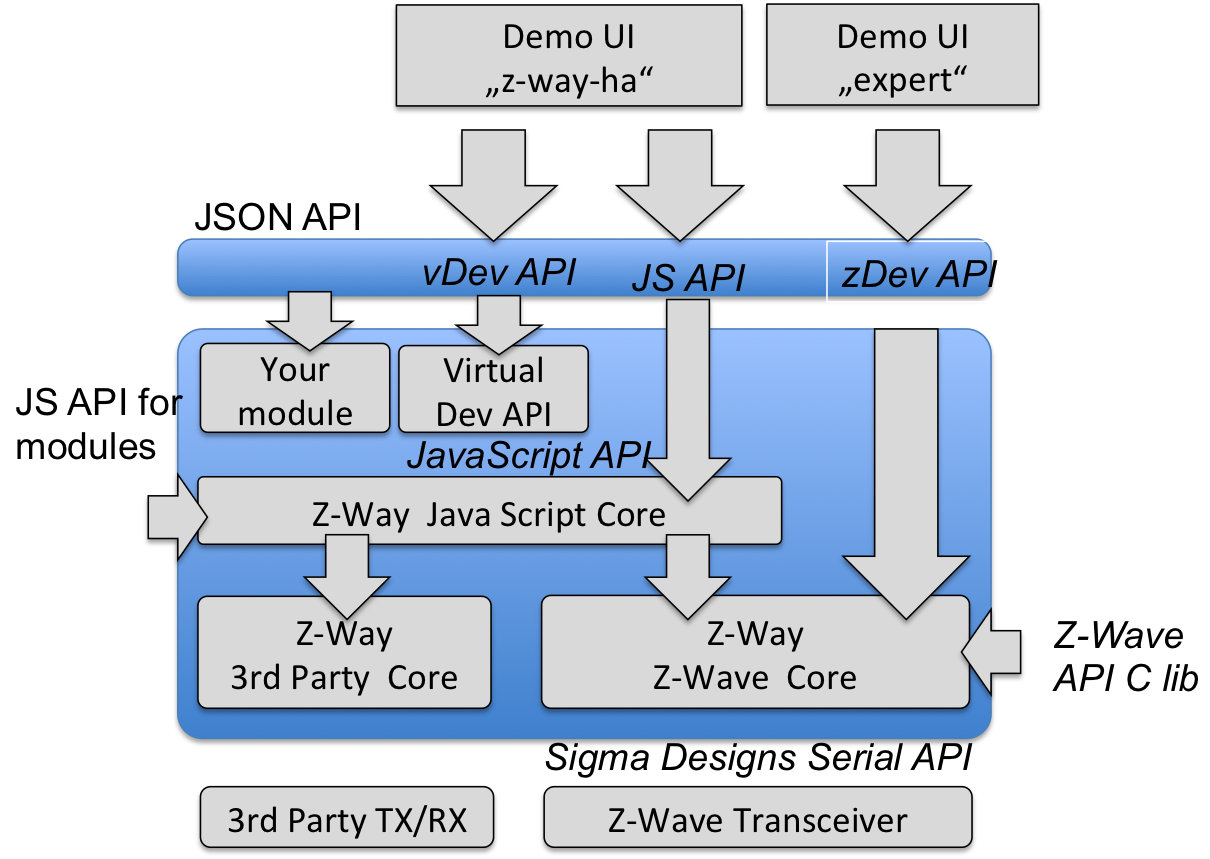
\includegraphics[scale=0.8]{pics/apis.png}
\caption{Z-Way APIs and their use by GUI demos}
\label{apis} 
\end{figure}

Z-Way offers multiple Application Programmers Interfaces (API) that are partly built on each other.
Figure \ref{apis} shows the general structure of Z-Way with focus on the APIs. The most important part of
Z-Way is the Z-Wave core. The Z-Wave core uses the standard
Sigma Designs Serial API to communicate with a Z-Wave compatible transceiver hardware but 
enhanced with some Z-Way specific functions such as Frequency Change. The standard
interface is not public but available for owners of the Sigma Designs Development Kit (SDK) 
\footnote{The Sigma Designs SDK is available from Digikey (www.digikey.com). Depending on the 
hardware options chosen the price varies between 2000 and 4000 USD} only.  

The Z-Wave core services can be accessed directly using the Z-Wave Device API (zDev API). There are two
Z-Wave Device API versions available:
\begin{itemize}
\item JSON API: All functions are available using a JSON API implemented by an 
embedded webserver. The "Expert" UI is using this interface and serves both as programmers 
and installers User Interface to operate the network and as reference implementation to demonstrate the use of this 
API. The Expert UI is completely written in AJAX Technology.
\item C Library API: All functions of the JSON API are available as C library 
function too. In the folder /z-way-devel there are all header files with the function 
prototypes. All function calls and the whole data model are identical. The URL

\paragraph{http://razberry.zwave.me/fileadmin/z-way-test.zip}

provides a sample application written in standard C that makes use of the C level API to 
demonstrate its application. Makefiles and project files for compilation on Linux and 
OSX are provided together with the sample code.

\end{itemize}

The \textbf{Z-Wave device API only allows the management of the Z-Wave network} and the control
and management of the devices as such. No higher order logic except the so called associations
between two Z-Wave devices can be used here.

For all \textbf{automation and higher order logic a Javascript automation engine} is available.
This engine is embedded in Z-Way can it be used to create your own home automation engine
working in addition or instead  of the Z-Way Home Automation engine. 
The implementation of the Java Script engine is organized in so called modules that implement 
a broad variety of applications using the underlying Z-Wave devices. The automation logic 
can also access and use other third party technology stacks such as the Enocean stack.

The Z-Way solution offers multiple prefabricated modules. \textbf{One of them implements
a Virtual Device API (vDev API)}. The virtual API unifies all information and control options
of the Z-Wave Device API, other third party API and own created virtual devices to simply
the access by AJAX based user interfaces.
The Demo GUI z-way-ha uses this API and demonstrates the use of the Virtual Device API.


\section{Quick Start}

The best way to learn about Z-Way is to use it. That is why the solutions comes with two
reference User Interfaces that can be accesses using a web browser. This allows to 
built, manage and use a first wireless smart home network with Z-Wave device (and/or with
devices using a third party wireless technology such as Enocean if supported by Z-Way) 
without writing a single line of code.
 
Once Z-Way is installed turn your browser to the URL

\paragraph{http://YOURIP:8083/expert}

\paragraph{or}

\paragraph{http://YOURIP:8083/z-way-ha} 

 
\paragraph{to use demonstation UIs available with Z-Way.} The port 8083 is predefined but can be 
changed  to any arbitrary port number by editing the file config.xml in the root folder
of Z-Way.

\begin{lstlisting}[caption=part of config.xml]{Name}
<config>
	...
	<port>8083</port>
 	...
</config>
\end{lstlisting}

In most cases you will want to control Z-Wave devices with Z-Way. Before a new device 
can be used, the device needs to be included in the Z-Wave network managed by Z-Way.
This management function is accessible in the Expert UI under the Tab 'Network'. 
Just hit the button "Include new Device" and then confirm the inclusion of the new device 
by hitting a button on the device or the specific action defined for this device to 
confirm inclusion.

You may need to refer to the manual of the new device for further information on how 
to confirm an inclusion by a controller.

The whole Expert UI is described in the Document 
\textbf{'Z-Way Expert User Interface Manual'} and therefore no scope of this document.


\section{API Overview}

All communication between the User Interfaces and Z-Way is handled using a 
web-technology-based  JSON interface provided by a built in web server.

There are different Application Programmers Interfaces available for Z-Way that serve 
different purposes:
\begin{enumerate}
\item Z-Wave Device API (zDev)
\item Third Party Technology APIs
\item JavaScript API
\item Virtual Device API/Business Logic API (vDev)
\end{enumerate}

\subsection{Z-Wave Device API}

The Z-Wave Device API implements the direct access to the Z-Wave network as such.
All Z-Wave devices are referred to by their unique identification in the wireless network - 
the Node Id. Z-Wave devices may have different instances of the same function, also 
called channels. The Z-Wave Device API refers to them as daughter objects of the 
physical device object identified by an instance Id. In case there only one instance the 
instance Id = 0  is used.

All device variables and available commands in a Z-Wave device are grouped in so called
command classes. The Z-Wave API allows direct access to all parameters, values and 
commands of these command class structures.

Beside the devices the Z-Wave Device API also offers access to the management interface
of the network. These functions are implemented as so called function classes within 
the object 'controller' or on the top level 'z-way' object.

The Z-Wave Device API can be accessed on the JSON API using the url path 



\paragraph{http://YOURIP:8083/ZWaveAPI/*}
\paragraph{Device objects or commands of these objects are accessed by} 
\paragraph{http://YOURIP:8083/ZWaveAPI/Run/devices[*].* }
\paragraph{http://YOURIP:8083/ZWaveAPI/Run/devices[x].instances[y].*}
\paragraph{http://YOURIP:8083/ZWaveAPI/Run/devices[x].instances[y].commandClasses[z].*} 
\paragraph{the whole data tree of the Z-Wave network is accessed using}  
\paragraph{http://YOURIP:8083/ZWaveAPI/Data/*}

\paragraph{
\textbf{Attention: The Installer UI is a complete reference of the Z-Wave API. It shows how 
to use all function it reveals the dynamics of the stack backend and visualizes all 
internal variables accessible on the API. }}

The chapter \ref{c2} describes the Z-Wave Device API in detail.

The section 'Function Classes' in chapter \ref{c2:fc} explains the different management 
functions and how they  can be used and will use the Expert UI dialogs as application example. The 
section 'Function Class Reference' in chapter \ref{FunctionClasses} all function 
classes available.

The control of devices  is implemented in Command Classes. The section 'Command Class 
Implementation' is again using certain dialogs of the Expert UI to explain how to access 
these functions. The chapter \ref{ccs} documents all 
command class functions. 

In order to access device and network related data in Z-Way, knowledge of the Z-Way 
data model is essential. The chapter \ref{datamodel} gives the necessary insight 
into the data model. All data of Z-Way are exposed on the Expert UI.

\subsection{Third Party Technology API}

Third party Technology APIs implement the same logic as the Z-Wave device API for other 
wireless technologies such as Enocean.

For more information  please refer to the technology specific descriptions.

\subsection{JavaScript API (JS API)}

The Z-Wave Device API or any other Third Party technology API do 
not offer any higher order logic support but the pure access to functions and parameters 
only.

Z-Way offers an automation engine to overcome this restriction. A server-side Javascript
Run time environment allows writing Javascript modules that are executed within Z-Way 
(means on the server). The same time all functions of the JS API can also be access on 
the client side (the web browser). This offers some cool debug and test capabilities. 
Among others it is possible to write whole JS functions right into the URL or the browser.

The JS API can be accessed from the web browser with the URL

\paragraph{http://YOURIP:8083/JS/Run/*}


\paragraph{Among others the whole Z-Wave Device API is available within the JS API using 
the object 'zway'.} As a result the following three statements refer to the 
very same function:

\begin{enumerate}
\item \textbf{http://YOURIP:8083/ZWaveAPI/Run/devices[3].*} Client Side URL access using 
the Z-Wave Device API.
\item \textbf{http://YOURIP:8083/JS/Run/zway.devices[3].*}: Client Side URL access 
using the JS API
\item \textbf{zway.devices[3].*}: Server Side access using the JS and the public zway object
\end{enumerate}

Due to the scripting nature of Javascript it is possible to 'inject' code at run time
using the interface. Here a nice example how to use the Java Script 
setInterval function:

\begin{lstlisting}[caption=Set Interval]{Name}
/JS/Run/setInterval(function() { 
	zway.devices[2].Basic.Get();
	}, 300*1000);
\end{lstlisting}

This code will, once 'executed' as URL within a web browser, call the Get() command
of the command class Basic of Node Id 2 every 300 seconds.  

A very powerful function of the JS API is the ability to bind functions to certain
values of the device tree. They get then executed when the value changes. Here is an 
example for this binding. The device No. 3 has a command class SensorMultilevel that offers
the variable level. The following call - both available on the client side 
and on the server side - will bind a simple alert function to the change of 
the variable.

\begin{lstlisting}[caption=Bind a function]{Name}
zway.devices[3].SensorMultilevel.data[1].level.bind( function() { 
	debugPrint('CHANGED\n'); 
	});  
\end{lstlisting}\footnote{Please note that the Sensor Multi Command class data is an array
index by the scale Id. Other command classes suc has Basic dont have this index but allow direct access using 
CommandClassName.data.val}

Chapter \ref{jsapi} and \ref{datamodel} describe the whole JS API in detail. The names 
and Ids of the different command classes as well as their instance variables can be found
in the Annex.

Javascript modules can and will generate new functions that are accessible using the 
JSON interface. For simplification function calls on the API (means on the client
side) are written in URL style starting with the word 'ZAutomation':

\begin{center}
ZAutomation/JSfunction/JParameter/
== JSfunction(JParameter)
\end{center}

\subsection{Virtual Device API}

One of the (server side) JavaScript modules already available is a mapping of all 
physical devices and functions into virtual devices. The purpose of this mapping is 
to simplify and to unify the implementation of a Graphical User Interface.

All functions and all instances of a physical device - that are represented as daughter
objects in the Z-Wave Device API -  are enrolled into individual virtual devices. 

In case the Z-Wave API shows one single physical device with two channels the virtual device 
API will show two devices with same function. In case the Z-Wave API shows a physical
device with  several different functions (like a binary switch and a analog sensor in one 
device) the Virtual Device API (vDev API) will show them as several devices with one 
function each.

The vDev is accessed using the JSON REST API but in a slightly different style. All 
devices, variables and commands are encoded into a URL style for easier handling in AJAX
code. A typical client side command in the vDev API looks like

\begin{center}

http://YOURIP:8083/ZAutomation/api/v1/devices/ZWayVDev\_6:0:37/command/off

\end{center}

'api' points to the vDev API function, 'v1' is just a constant to allow future extensions. 
The devices are referred by a name that is automatically generated from the Z-Wave 
Device API. The vDev also unifies the commands 'command' and the parameters, here 'off'.

On the server side the very same command would be encoded in a JavaScript style.

\begin{center}
	dev = this.controller.devices,get('ZWayVDev\_6:0:37');
	dev.command('off');
\end{center}

The vDev API also offers support for notifications, locations information, the use of other
modules etc. For details please refer to Chapter \ref{vdev}.

\subsection{Comparison}

Table \ref{c1:comp} summarizes the functions of the different APIs.


\begin{table}
\begin{tabular}{|p{40mm}|p{50mm}|p{20mm}|p{20mm}|}
\hline
API Type &	Core Function & Network Management & Automation\\
\hline
Z-Wave Dev API (JSON)	& Access to physical network and physical devices via JSON	&
Yes	&No\\
\hline
Z-Wave Dev API (C lib) 	& Access to physical network and physical devices via C style calls &
Yes	&No\\
\hline
JavaScript API & Access to physical network and devices plus JS type functions	&
No	&Yes, via zDev\\
\hline
vDev API & Unified Access to functions of devices, optimized for AJAX GUI&
No	&Yes\\
\hline
\hline
\end{tabular}
\caption{Different APIs of the Z-Way system} 
\label{c1:comp}
\end{table}		

For demo and sample code please refer to the following sources:

\begin{enumerate}
\item \textbf{Z-Wave Device API JSON} Expert UI on http://YOURIP:8083/expert
\item \textbf{Z-Wave C Library API} Header files in folder /z-way-devel 
\item \textbf{Javascript API} Modules in folder /automation
\item \textbf{vDev API} z-way-ha UI on http://YOURIP:8083/z-way-ha
\end{enumerate}




 